\documentclass{article}
%% Oh yes. TIKZ pictures / graphs
%% -------------------------------------
\usepackage{tikz}
\usepackage{pgfplots}
\usepackage{tikz-3dplot}
\usetikzlibrary{calc,fadings,decorations.pathreplacing,shadings,intersections,backgrounds,arrows}
\usetikzlibrary{arrows,positioning,shapes,backgrounds,fit} 
\usepackage{verbatim}
\definecolor{MyBrightBlue}{rgb}{1,0.5,0}
\definecolor{airforceblue}{rgb}{0.36, 0.54, 0.66}
\definecolor{MyBlue}{rgb}{0.61, 0.87, 1.0}
\definecolor{Karminrot}{RGB}{165, 30, 55}

%% This is when making tikz plots
%% -------------------------------------
\pgfplotsset{rdstyle/.style={%
        width=8cm,
        ylabel={y},
        xlabel={x},
        xmin=-2,xmax=3,
        xtick={-2,-1,...,3}}}
%% -------------------------------------




\begin{document}

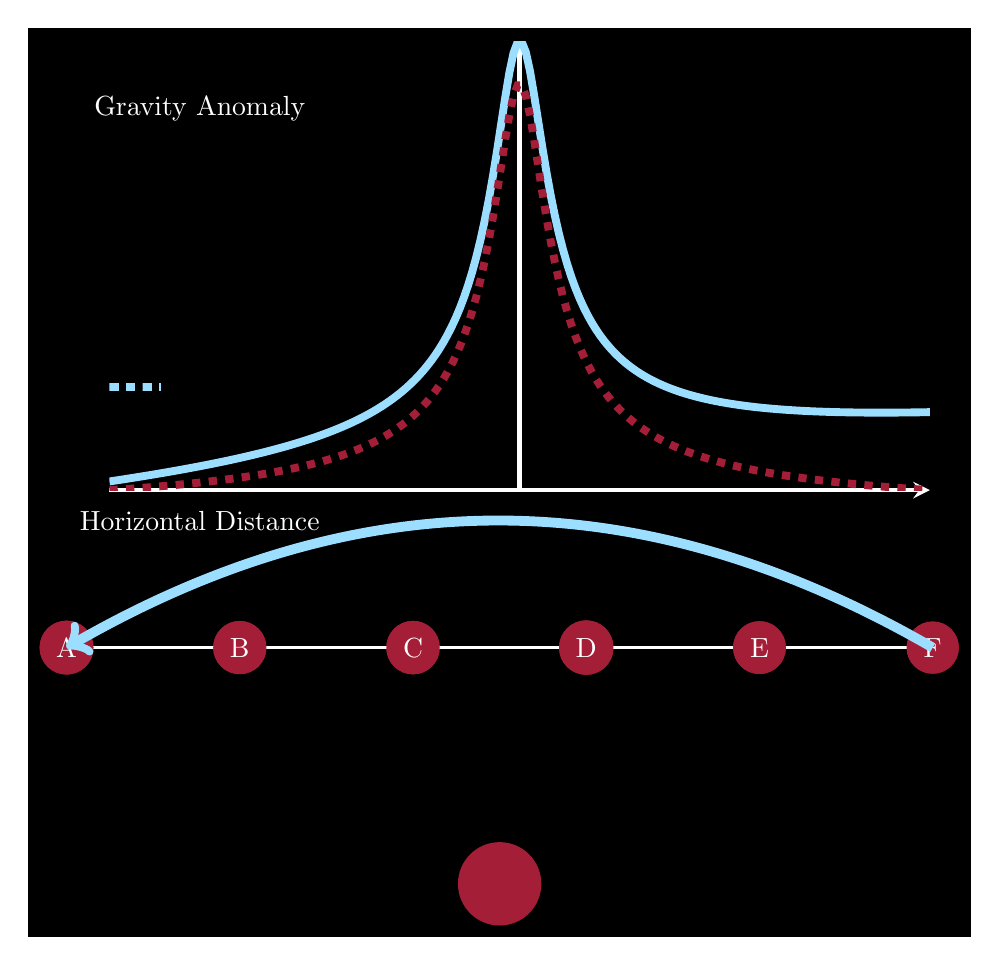
\begin{tikzpicture}[background rectangle/.style={fill=black},show background rectangle]
    \coordinate (TL) at (-2,-2);
    \coordinate (TR) at (9,-2);
    \coordinate (BL) at (-2,-10);
    \coordinate (BR) at (9,-10);
    \coordinate (Target) at (3.5,-5);

    %\draw[arrow](TL.west) to [out=190,in=170] node[above]{Flow: $\alpha$ } (TR.west);

    %\node[circle] (TL) {}

    \draw [->,thick,white] (TL) -- (TR) node[circle,fill=Karminrot,pos=0]{A} node[circle,fill=Karminrot,pos=0.2]{B} node[circle,fill=Karminrot,pos=0.4]{C} node[circle,fill=Karminrot,pos=0.6]{D} node[circle,fill=Karminrot,pos=0.8]{E} node[circle,fill=Karminrot,pos=1.0]{F};
    \draw [->,thick,white] (TL) -- (TR) node[circle,fill=Karminrot,pos=0]{A} node[circle,fill=Karminrot,pos=0.2]{B} node[circle,fill=Karminrot,pos=0.4]{C} node[circle,fill=Karminrot,pos=0.6]{D} node[circle,fill=Karminrot,pos=0.8]{E} node[circle,fill=Karminrot,pos=1.0]{F};
    %\node[circle,draw] (Target) at (Target){};
    \fill[Karminrot] (Target) circle (3.5ex);
    \draw [<-,line width=1.25mm,MyBlue]  (TL) to[out=30,in=150] (TR);
    \begin{axis}[
        ylabel={Gravity Anomaly},
        xlabel={Horizontal Distance},
        label style={font=\normal},
        axis lines=middle, xtick=\empty,ytick=\empty,
        color=white,
        width=12cm,
        height=\axisdefaultheight,
        at={(0.-0.12\linewidth,0)},
        axis line style=ultra thick,
        x label style={at={(axis description cs:0.11,-0.025)},anchor=north},
        y label style={at={(axis description cs:0.11,0.9)},anchor=north}
           ]
        \addplot[domain=-80:80,samples=200,color=MyBlue,line width=1.0mm] {5/((25+x*x)^(0.5)*1000)+x/1000000+1/10000};
        \addplot[domain=-80:80,samples=200,color=Karminrot,line width=1.0mm,dashed] {5/((25+x*x)^(0.5)*1000)};
        \addplot[domain=-80:-70,samples=200,color=MyBlue,mark=-*,line width=1.0mm,dashed] {x*0.0+3/10000};
      \end{axis}
  \end{tikzpicture}

\end{document}